% Generated by code/ch10_complexity.py -- do not edit by hand.
\definecolor{qocA}{rgb}{0.00,0.45,0.70}
\definecolor{qocB}{rgb}{0.90,0.60,0.00}
\definecolor{qocC}{rgb}{0.00,0.62,0.45}
\definecolor{qocD}{rgb}{0.80,0.40,0.00}
\definecolor{qocE}{rgb}{0.80,0.60,0.70}
\definecolor{qocF}{rgb}{0.35,0.70,0.90}
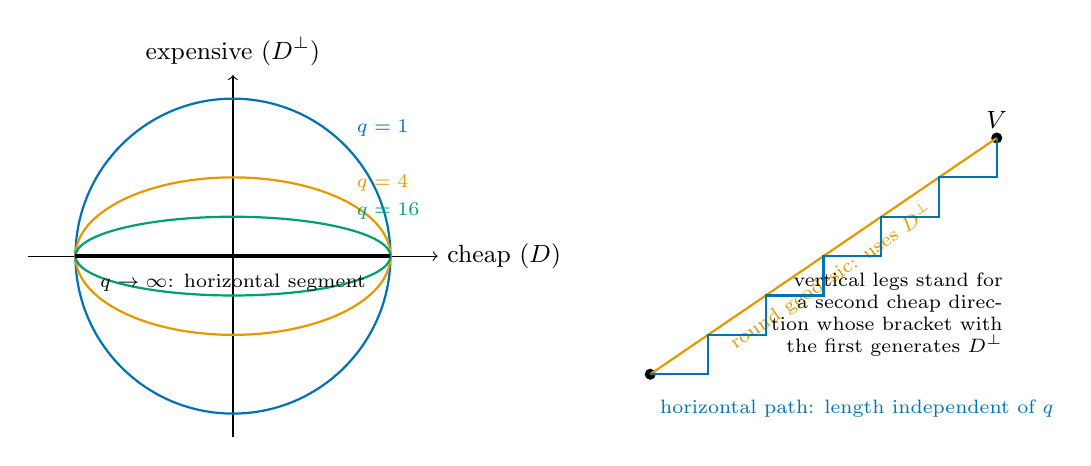
\begin{tikzpicture}[]
\begin{scope}
\draw[->] (-2.6,0) -- (2.6,0) node[right,font=\small] {cheap ($D$)};
\draw[->] (0,-2.3) -- (0,2.3) node[above,font=\small] {expensive ($D^\perp$)};
\draw[thick,qocA] (0,0) ellipse (2 and 2.000);
\node[qocA,font=\scriptsize,anchor=south west] at (1.45,1.40) {$q=1$};
\draw[thick,qocB] (0,0) ellipse (2 and 1.000);
\node[qocB,font=\scriptsize,anchor=south west] at (1.45,0.70) {$q=4$};
\draw[thick,qocC] (0,0) ellipse (2 and 0.500);
\node[qocC,font=\scriptsize,anchor=south west] at (1.45,0.35) {$q=16$};
\draw[very thick,black] (-2,0) -- (2,0);
\node[font=\scriptsize,anchor=north] at (0,-0.1) {$q\to\infty$: horizontal segment};
\end{scope}
\begin{scope}[xshift=7.5cm]
\fill (-2.2,-1.5) circle (2pt) node[below,font=\small] {$\Id$};
\fill (2.2,1.5) circle (2pt) node[above,font=\small] {$V$};
\draw[thick,qocB] (-2.2,-1.5) -- (2.2,1.5);
\node[qocB,font=\scriptsize,rotate=34] at (0.1,-0.25) {round geodesic: uses $D^\perp$};
\draw[thick,qocA] (-2.200,-1.500) -- (-1.467,-1.500) -- (-1.467,-1.000) -- (-0.733,-1.000) -- (-0.733,-0.500) -- (0.000,-0.500) -- (0.000,0.000) -- (0.733,0.000) -- (0.733,0.500) -- (1.467,0.500) -- (1.467,1.000) -- (2.200,1.000) -- (2.200,1.500);
\node[qocA,font=\scriptsize,anchor=north west] at (-2.2,-1.7) {horizontal path: length independent of $q$};
\node[font=\scriptsize,anchor=south east,text width=3.6cm,align=right] at (2.4,-1.4) {vertical legs stand for a second cheap direction whose bracket with the first generates $D^\perp$};
\end{scope}
\end{tikzpicture}
